\section{Methodology}
\label{sec:methodology}
Underwater images distorted by color or circumstance lack ground truth, which is a necessity for previous colorization
approaches. Furthermore, the distortion present in an underwater image is highly nonlinear; simple methods such as
adding a hue to an image do not capture all of the dependencies. We propose to use CycleGAN as a distortion model in
order to generate paired images for training. Given a domain of underwater images with no distortion, and a domain of
underwater images with distortion, CycleGAN is able to perform style transfer. Given an undistorted image, CycleGAN
distorts it such that it appears to have come from the domain of distorted images. These pairs are then used in our
algorithm for image reconstruction.

\subsection{Dataset Generation}
Depth, lighting conditions, camera model, and physical location in the underwater environment are all factors that affect the 
amount of distortion an image will be subjected to. Under certain conditions, it is possible that an underwater image may have 
very little distortion, or none at all. We let 
$I^C$ be an underwater image with no distortion, and $I^D$ be the same image with distortion. Our goal is to learn the function 
$f: I^D \rightarrow I^C$. Becasue of the difficulty of collecting underwater data, more often than not only $I^D$ or $I^C$ exist, 
but never both.

To circumvent the problem of insufficient image pairs, we use CycleGAN to generate $I^D$ from $I^C$, which gives us a 
paired dataset of images. Given two datasets $X$ and $Y$, where $I^C \in X$ and $I^D \in Y$, CycleGAN learns a mapping $F: X 
\rightarrow Y$. Figure~\ref{fig:cgan_samples} shows paired samples generated from CycleGAN. From this paired dataset we train a 
generator $G$ to learn the function $f: I^D \rightarrow I^C$. It should be noted that during our data generation process, CycleGAN 
simultaneously learns a mapping $G: Y \rightarrow X$, which is similar to $f$. In Section~\ref{sec:experiments}, we compare images 
generated by CycleGAN with images generated through our approach.

\subsection{Adversarial Networks}
\label{sec:gans}
\nostarnote{check this paragraph as I added some more text}In machine learning literature, Generative Adversarial Networks 
(GANs)~\cite{goodfellow2014generative} represent a class of generative models based on game theory in which a generator network 
competes against an adversary. From a classification perspective, the generator network produces instances which actively attempt 
to `fool' the discriminator network. The goal is for the discriminator network to be able to distinguish between `true' 
instances coming from the dataset and `false' instances produced by the generator network.
%, and thus improve its classification accuracy.
In our case, conditioned on an image $I^D$, the generator is trained to produce an image to try and fool the 
discriminator, which is trained to distinguish between distorted and non-distorted underwater images. In the original
GAN formulation, our goal is to solve the minimax problem:

\begin{figure}
\vspace{2mm}
\centering
\begin{tabular}{p{1.7cm} p{1.7cm} p{1.7cm} p{1.7cm}}
   
   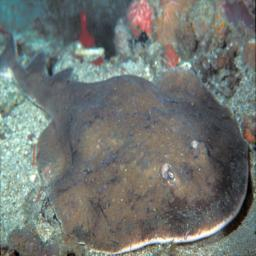
\includegraphics[width=0.8in]{n01496331_873_X} &
   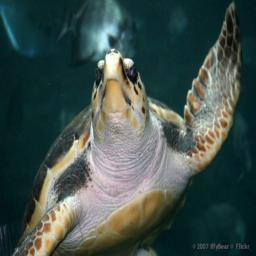
\includegraphics[width=0.8in]{n01664065_4022_X} &
   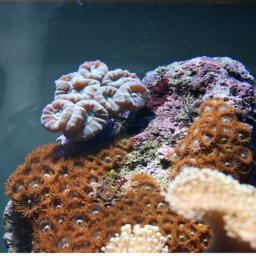
\includegraphics[width=0.8in]{n01917289_889_X} &
   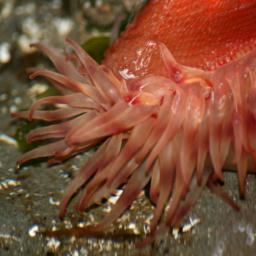
\includegraphics[width=0.8in]{n01914609_116_X} \\
   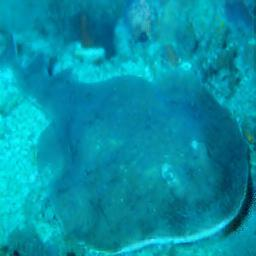
\includegraphics[width=0.8in]{n01496331_873_Y} &
   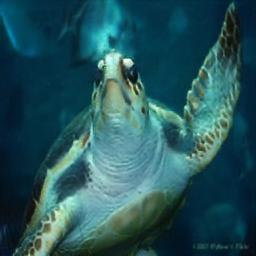
\includegraphics[width=0.8in]{n01664065_4022_Y} &
   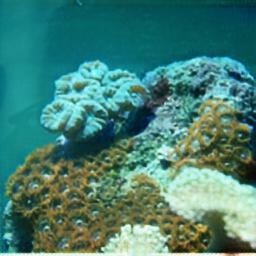
\includegraphics[width=0.8in]{n01917289_889_Y} &
   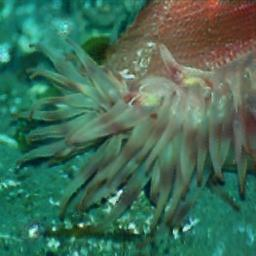
\includegraphics[width=0.8in]{n01914609_116_Y} \\

\end{tabular}
\caption{Paired samples of ground truth and distorted images generated by CycleGAN. Top row: Ground truth.
Bottom row: Generated samples.}
\label{fig:cgan_samples}
\vspace{-5mm}
\end{figure}


\begin{equation}
\begin{aligned}
   \min\limits_{G}\max\limits_{D} \mathbb{E} & _{I^C \sim p_{train}(I^C)} [logD(I^C)] + \\
   \mathbb{E} & _{I^D \sim p_{gen}(I^D)}[log(1 - D(G(I^D)))]
\end{aligned}
\end{equation}

Note for simplicity in notation, we will further omit $I^C \sim p_{train}$ and $I^D \sim p_{gen}$. In this formulation, 
the discriminator is hypothesized as a classifier with a sigmoid cross-entropy loss function, which in practice may lead
to issues  such as the vanish gradient and mode collapse. As shown by \cite{arjovsky2017towards}, as
the discriminator improves, the gradient of the generator vanishes, making it difficult or impossible to train. Mode
collapse occurs when the generator ``collapses'' onto a single point, fooling the discriminator with only one instance.
To illustrate the effect of mode collapse, imagine a GAN is being used to generate digits from the MNIST~\cite{lecun2010mnist} 
dataset, but it only generated the same digit. In reality, the desired outcome would be to generate a diverse collection of all 
the digits.
There have been a number of recent methods which hypothesize a different loss function for the discriminator
\cite{mao2016least,arjovsky2017wasserstein,gulrajani2017improved,zhao2016energy}. We focus on the Wasserstein GAN
(WGAN) \cite{arjovsky2017wasserstein} formulation, which proposes to use the Earth-Mover or \textit{Wasserstein-1}
distance $W$ by constructing a value function using the Kantorovich-Rubinstein duality \cite{villani2008optimal}.
In this formulation, $W$ is approximated given a set of $k$-Lipschitz functions $f$ modeled as neural networks. To
ensure $f$ is $k$-Lipschitz, the weights of the discriminator are clipped to some range $[-c, c]$. In our work, we
adopt the Wasserstein GAN with gradient penalty (WGAN-GP) \cite{gulrajani2017improved}, which instead of clipping
network weights like in \cite{arjovsky2017wasserstein}, ensures the Lipschitz constraint by enforcing a soft
constraint on the gradient norm of the discriminator's output with respect to its input. Following
\cite{gulrajani2017improved}, our new objective then becomes

\begin{equation}
\begin{aligned}
   \mathcal{L}_{WGAN}(G,D) = \mathbb{E} [D(I^C)] - \mathbb{E} & [D(G(I^D))] + \\
   \lambda_{GP} \mathbb{E} & _{\hat{x} \sim \mathbb{P}_{\hat{x}}} [(|| \nabla_{\hat{x}} D(\hat{x})||_2 -1)^2 ],
\end{aligned}
\end{equation}

%\begin{equation}
%\begin{aligned}
%   \mathcal{L}_{GAN} = \mathbb{E}_{I^D \sim p_{gen}(I^D)} [D(I^D)] - \mathbb{E} & _{I^C \sim p_{train}(I^C)} [D(I^C)] + \\
%   \lambda \mathbb{E} & _{\hat{x} \sim \mathbb{P}_{\hat{x}}} [(|| \nabla_{\hat{x}} D(\hat{x})||_2 -1)^2 ].
%\end{aligned}
%\end{equation}

\noindent where $\mathbb{P}_{\hat{x}}$ is defined as samples along straight lines between pairs of points coming from
the true data distribution and the generator distribution, and $\lambda_{GP}$ is a weighing factor. In order to give $G$
some sense of ground truth, as well as capture low level frequencies in the image, we also consider the $L1$ loss

\begin{equation}
   \mathcal{L}_{L1} = \mathbb{E} [ || I^C - G(I^D) ||_1 ].
\end{equation}
%\begin{equation}
%   \mathcal{L}_{L1} = \mathbb{E}_{I^D \sim p_{gen}, I^C \sim p_{train}} [ || I^C - G(I^D) ||_1 ].
%\end{equation}

\noindent Combining these, we get our final objective function for our network, which we call Underwater GAN (UGAN),

\begin{equation}
   \begin{aligned}
      \mathcal{L}_{UGAN}^* = \min\limits_{G}\max\limits_{D} \mathcal{L}_{WGAN}(G,D) + \lambda_{1} \mathcal{L}_{L1}(G).
   \end{aligned}
\end{equation}


\subsection{Image Gradient Difference Loss}
Often times generative models produce blurry images. We explore a strategy to sharpen these predictions by
directly penalizing the differences of image gradient predictions in the generator, as proposed by
\cite{mathieu2015deep}. Given a ground truth image $I^C$, predicted image $I^P = G(I^D)$, and $\alpha \geq 1$, the
Gradient Difference Loss (GDL) is given by

\begin{equation}
   \begin{aligned}
      \mathcal{L}_{GDL}(I^C, I^P) = \\ \sum\limits_{i,j} || & I^C_{i,j} - I^C_{i-1,j}| - | I^P_{i,j} - I^P_{i-1,j}||^{\alpha} + \\
      || & I^C_{i,j-1} - I^C_{i,j}| - | I^P_{i,j-1} - I^P_{i,j}||^{\alpha}.
   \end{aligned}
   \label{gdl_eq}
\end{equation}

\noindent In our experiments, we denote our network as UGAN-P when considering the GDL, which can be expressed as
%\starnote{JS: DONE. I don't like the - in this equation, but don't know how to change it to be shorter}

\begin{equation}
   \begin{aligned}
      \mathcal{L}_{UGAN\scalebox{0.4}[1.0]{\( - \)}P}^* = \min\limits_{G}\max\limits_{D} \mathcal{L}_{WGAN}(G,D) + & \\
      % \mathcal{L}_{UGAN-P}^* = \min\limits_{G}\max\limits_{D} \mathcal{L}_{WGAN}(G,D) + & \\
      \lambda_{1} \mathcal{L}_{L1}(G) + & \lambda_{2} \mathcal{L}_{GDL}
   \end{aligned}
\end{equation}


\subsection{Network Architecture and Training Details}
Our generator network is a fully convolutional encoder-decoder, similar to the work of \cite{isola2016image}, which is
designed as a ``U-Net'' \cite{ronneberger2015u} due to the structural similarity between input and output.
Encoder-decoder networks downsample (encode) the input via convolutions to a lower dimensional embedding, in which
this embedding is then upsampled (decode) via transpose convolutions to reconstruct an image. The advantage of using
a ``U-Net'' comes from explicitly preserving spatial dependencies produced by the encoder, as opposed to relying on the
embedding to contain all of the information. This is done by the addition of ``skip connections'', which concatenate
the activations produced from a convolution layer $i$ in the encoder to the input of a transpose convolution layer
$n-i+1$ in the decoder, where $n$ is the total number of layers in the network. Each convolutional layer in our
generator uses kernel size $4 \times 4$ with stride 2. Convolutions in the encoder portion of the network are followed
by batch normalization \cite{pmlr-v37-ioffe15} and a leaky ReLU activation with slope $0.2$, while transpose
convolutions in the decoder are followed by a ReLU activation \cite{nair2010rectified} (no batch norm in the decoder).
Exempt from this is the last layer of the decoder, which uses a TanH nonlinearity to match the input distribution of
$[-1, 1]$. Recent work has proposed Instance Normalization \cite{ulyanov2016instance} to improve quality
in image-to-image translation tasks, however we observed no added benefit.

Our fully convolutional discriminator is modeled after that of \cite{radford2015unsupervised}, except no batch
normalization is used. This is due to the fact that WGAN-GP penalizes the norm of the discriminator's gradient with
respect to each input individually, which batch normalization would invalidate. The authors of
\cite{gulrajani2017improved} recommend layer normalization \cite{ba2016layer}, but we found no significant improvements.
Our discriminator is modeled as a PatchGAN \cite{isola2016image,li2016precomputed}, which discriminates at the level of
image patches. As opposed to a regular discriminator, which outputs a scalar value corresponding to real or fake, our
PatchGAN discriminator outputs a $32 \times 32 \times 1$ feature matrix, which provides a metric for high level
frequencies. %which is combinied with the low level frequencies from the $L1$ loss.
